\documentclass[autodetect-engine,dvipdfmx-if-dvi,ja=standard,a4paper,12pt,twoside,openany,layout=v2]{bxjsbook}
%\usepackage{reviewmacro}
\usepackage{localst17}
\usepackage{mymintedsetting}
\usepackage{lipsum}

\title{知らねー}
\author{うっひょい \and ちくうぇいと \and あわあわ \and けんつ \and さわだ \and Jumpaku}
\date{\today}

\begin{document}
\begin{titlepage}
  
\includegraphics{main.jpg}
\end{titlepage}
\maketitle
\frontmatter
\chapter{はじめに}
hogehuga


\tableofcontents
\mainmatter
\chapterauthor{うっひょい}
\chapter{\LaTeX の乱数生成アルゴリズムを改善する}
\section{乱数とは}
\subsection{疑似乱数と真の乱数}
\subsection{準乱数とは}

\section{乱数生成コマンド}
\LaTeX のパッケージに固定小数演算ができるFPパッケージがあります.
\subsection{固定小数演算}
\TeX ,\LaTeX は共に整数の演算は可能ですが,小数点を含む計算は行うことができません(寸法を除く).
固定小数点の演算をすることを目的としてあるのがFPパッケージです.
\subsection{乱数を出力するFPrandomコマンド}
fpパッケージの中には上記以外にも$0\sim 1$の範囲の疑似乱数を出力するFPrandomというコマンドがあります.
FPseedでシード値を決めてからFPrandomを使って変数に乱数を格納します.
\begin{texcode}
\FPseed = 156
\FPrandom{\result}
\FPprint{\result}
\end{texcode}

\section{FPrandomの乱数生成アルゴリズムを調べる}
\subsection{目的}
今回はFPrandomに使われている疑似乱数がいわゆる多くの問題点がある昔のアルゴリズムかどうかを調べる為に行います.

\subsection{疑似乱数アルゴリズムの問題点}
現在,世に出回っている疑似乱数アルゴリズムは様々あります.
これは今まで研究されてきたアルゴリズムに何かしらの問題があるからです.
偏りが出たり,パターンがあったり様々です.
また,疑似乱数には周期があります.一定の数の乱数を出力したらまた,最初から同じ疑似乱数列を出力し始めます.
現在は計算機のスペックも高くなりより複雑なシミュレーションを行えるようになりました.
その為,用いられる疑似乱数の数が従来のアルゴリズムでは周期を上回る危険性もありました.
周期を伸ばすことも新しい疑似乱数アルゴリズムを開発する理由の一つです.

\subsection{ソースを読む}
それではfpパッケージのソースを読んでいきます.
しかし,実際にはfpパッケージ本体が内部的に呼び出しているfp-randomパッケージのソースを読んでいきます.

\subsubsection{コメントに正解が書いてあった}
22行目からFPrandomの定義が始まります.その直後,コメントが長く続いています.
コメントには次のようなことが書かれていました.
\begin{quote}
Algorithm reproduce from a very old Fortran program (unknown origin!)
\end{quote}
どうやら大昔のFortranの疑似乱数アルゴリズムを\TeX に起こしたものがFPrandomの正体みたいですね.
これはいろいろ問題点がありそうですね.
更にその下のコメントにはFortranで書かれた疑似乱数アルゴリズムらしきものがあります.
これを読んでいけばどんなアルゴリズムが使われているか分かりますがそれではつまらないので
コメントを抜けた後の\TeX で書かれた疑似乱数アルゴリズムの方を見ていきましょう.

\subsubsection{\TeX のマクロで実装された疑似乱数アルゴリズム}
\begin{texcode}
\ifnum\FPseed=0%
     \FPseed=123456789%
     \FP@debug{random: seed value undefined! We will used \the\FPseed.%
        Define it if you want to generate a different sequence of random numbers.}%
\else%
     \FP@debug{random: seed value used: \the\FPseed}%
\fi%
\end{texcode}
これはシードを指定してるかどうかを判定してしてない場合123456789をシードとするというマクロですね.
次見ていきます.
\begin{texcode}
\FP@xia=\FPseed%
\divide\FP@xia by 127773%
\FP@xib=\FP@xia%
\multiply\FP@xib by 127773%
\advance\FP@xib by -\FPseed%
\FP@xib=-\FP@xib%
\multiply\FP@xia by 2836%
\FPseed=\FP@xib%
\multiply\FPseed by 16807%
\advance\FPseed by -\FP@xia%
\end{texcode}
このアルゴリズムのコアとなる乱数の計算ですね.\TeX で書いてる為ごちゃごちゃしていますが
数式で表すと以下のようになります.

\[
S_{n+1} = - \frac{S_n}{127773}\times 2836 + (16807S_n \bmod 127773)
\]
{\LARGE 二重で線形合同法}
$S_n$が$n$番目に出力した乱数で$S_{n+1}$は$n+1$番目に出力する乱数です.つまり漸化式になっています.
線形合同法の漸化式と似ていますね.
線形合同法はC言語のrand関数に採用されているアルゴリズムですが多くの問題点が発見されていて現在は非推奨となっています.
線形合同法では$16807S_n$の部分が定数ですが,それが乱数を含む形になっています.
線形合同法の式は以下のとおりです.

\[
S_{n+1}=(A\times S_n + B) \bmod M \quad \textrm{(A,B,Mは定数)}
\]

...構造が非常に似ていますね.

\begin{texcode}
 \ifnum\FPseed>0%
  \else%
      \advance\FPseed by 2147483647%
  \fi%
  \FPdiv\FP@tmpa{\the\FPseed}{2147483647}%
  \global\let\FP@tmp\FP@tmpa%
  \global\FPseed=\FPseed%
\end{texcode}
乱数の正規化を行っています.$2147483647(=2^{32}-1)$がこの乱数列における最大値$M$で
この時点で$n+1$番目の乱数が負の値の場合は$M$を乱数に足します.
その後FPdivと呼ばれる小数の割り算ができるマクロによって乱数を$M$で割り,乱数を$0\sim 1$の範囲の値に正規化しています.
\begin{texcode}
  \let#1\FP@tmp%
\end{texcode}
最後に,FPrandomの第一引数に算出した乱数を代入して終了です.
\subsubsection{実際に出力してみる}
前節でFPrandomは線形合同法が用いられていることが分かりました.
しかし,線形合同法は実装が簡単にできる分,構造が単純で,
偏りが出たり,周期が短いことが問題となっています.
この節では,その問題点がFPrandomコマンドにも起こり得ることを検証していきます.
まずは周期性ですが,線形合同法の周期は$M-1$です.
FPrandomは$M=214793647$なので周期は$214793646$となります.
つまり,FPranndomコマンドを$M$回呼び出すと最初の乱数と一致することになります.


\chapterauthor{chikuwait(ちくうぇいと)}
\chapter{超入門 仮想化技術}
\input{chikuwa_IT}

\chapterauthor{あわあわ}
\chapter{ほげ}
\input{materialofmouse}

\chapterauthor{けんつ}
\chapter{ほげ}
\section{はじめに}
このセクションではLinux Kernelに対する知見をカーネルモジュール制作を通して深めることを目的としています。
単純なカーネルモジュールを制作してもあまり意味が無いので、ここではカーネルモジュールとして動作するEchoサーバを作ることを題材にします。

\subsection{カーネルモジュールとは}
カーネルモジュールとは、Linux上で動的につまりは起動中でも追加削除可能なモジュールを指す。
通常のOSではカーネルにモジュールを追加するとカーネルそのものを再構築する必要がでてくるが、Linuxカーネルモジュールはそれを必要とせずにモジュールの追加、利用、削除が可能となっている。
ここで紹介するカーネルモジュールはその特性上、ローダブルカーネルモジュールと呼ばれることがある。
現在ロードされているカーネルモジュールを確かめるには\mintinline{bash}{lsmod}で確認することができる。

\subsection{カーネルからHello,World!!}

\subsection{}


\chapterauthor{さわだ}
\chapter{自作エディタ入門編}
\section{はじめに}
皆さんはちょっとしたメモやプログラミングにどんなエディタを使いますか?Vim?それともEmacs?まぁ色々ありますよね.人それぞれ好き嫌いがあると思います.僕はVimを自分好みに拡張するのが好きです\footnote{そこのEmacs教徒,石を投げないで!}.でも,人には自作欲求があります.CPU,OS,言語,更に最近はキーボードなどが人気ですが,エディタも中々面白いですよ.CUIは時代遅れなんてそんなの気にしちゃいけません.ソースコードは\href{https://github.com/takuzoo3868/takdit}{github.com/takuzoo3868/takdit}に置いてあります.

\section{準備}
テキストエディタと言いつつも初めから高機能なエディタを自作するのは至難の業です.そこで,最低限ファイルを編集して保存できるようにする所から始めるといいかなと思います.次にシンタックスハイライト対応や文字列検索機能などを考えていきましょう.リポジトリにあるテキストエディタのファイル構造は以下ようになっています.
\begin{figure}[H]
  \dirtree{%
  .1 takdit/.
  .2 modules/ \dotfill  \begin{minipage}[t]{7cm}拡張機能を追加していくディレクトリ{.}\end{minipage}.
  .3 syntax/ \dotfill  \begin{minipage}[t]{7cm}シンタックスハイライト用の構造体を定義{.}\end{minipage}.
  .2 LICENSE.
  .2 Makefile.
  .2 README.md.
  .2 takdit.c \dotfill  \begin{minipage}[t]{7cm}メインとなるソースコード{.}\end{minipage}.
  .2 takdit.h \dotfill  \begin{minipage}[t]{7cm}定数定義や構造体を含むヘッダ{.}\end{minipage}.
  }
\end{figure}
外部ライブラリに依存しない事を目標としていますが,Cコンパイラと\mintinline{bash}{make}コマンドは準備する必要があります.
\mintinline{bash}{cc --version}や\mintinline{bash}{make -v}でインストールされているかどうか確認できます.自身の環境にコンパイラがインストールされていなかった場合は,Google先生に聞いてみましょう.

\subsubsection{makeによるコンパイル}
解説のために本文中では\mintinline{bash}{takdit}と記載しますが,好きな名前に置き換えて下さい\footnote{4文字程度が打ちやすくていい感じです.私は馬鹿なので6文字も使ってしまいました.}.\mintinline{bash}{cc takdit.c -o takdit}などと打ち込めばコンパイルできます.しかし試行錯誤を繰り返すため,再コンパイルの度に同じ事をするのはあまりスマートではありません.\mintinline{bash}{make}を用いることでプログラムコンパイルを少しだけ楽にしておきましょう.\mintinline{bash}{Makefile}を作成し,以下の内容を記述しておきます.
\begin{minted}[frame=lines,framesep=2mm,baselinestretch=1.2,fontsize=\footnotesize,linenos,breaklines]{text}
  takdit: takdit.c
  $(CC) -o takdit takdit.c -Wall -W -pedantic -std=c99
\end{minted}
この辺については,準備段階なので詳細は省きます.とてもざっくりに言いますと,諸々の構文をチェックして警告を表示してくれるようオプションを設定しています.これで準備は完了です.

\section{基本構成}
基本となる骨格はkiloというテキストエディタを参考にします\footnote{\href{https://github.com/antirez/kilo}{github.com/antirez/kilo}}.
Salvatore Sanfilippo氏によって開発されたC言語製のエディタです.BSD 2-clauseにて公開されています.
紹介文に,
\begin{quote}
  Kilo is a small text editor in less than 1K lines of code (counted with cloc).
\end{quote}
とあるように1000行程度なので目で追っていくもの問題ないでしょう.ちょっと厳しいという方は\mintinline{c}{int main()}だけでも目を通す事をお勧めします.
\inputminted[frame=lines,framesep=2mm,baselinestretch=1.2,fontsize=\footnotesize,linenos,breaklines]{c}{takuzoo3868asset/main.c}
処理の流れはコメントにあるように,
\begin{enumerate}
  \item 起動にあたりエディタの初期化
  \item 引数にあるファイルの拡張子に対応したシンタックスハイライトを適用
  \item ファイルをメモリ上へ展開
  \item エスケープシーケンスを利用してターミナルをRawモードへ変更
  \item ループ処理
\end{enumerate}
となります.ループでは画面反映とキー入力待ちを行っています.本書では基本構造として上記の5点を解説します.
編集対象ファイルの内容をメモリに読み込み,一つの文字列データとして確保\footnote{\mintinline{c}{char*}でアクセスされるヒープ上のメモリ領域}.

 \inputminted[frame=lines,framesep=2mm,baselinestretch=1.2,fontsize=\footnotesize,linenos,breaklines]{c}{takuzoo3868asset/struct.c}

 \inputminted[frame=lines,framesep=2mm,baselinestretch=1.2,fontsize=\footnotesize,linenos,breaklines]{c}{takuzoo3868asset/initEditor.c}

 \inputminted[frame=lines,framesep=2mm,baselinestretch=1.2,fontsize=\footnotesize,linenos,breaklines]{c}{takuzoo3868asset/editorSelectSyntaxHighlight.c}

 \inputminted[frame=lines,framesep=2mm,baselinestretch=1.2,fontsize=\footnotesize,linenos,breaklines]{c}{takuzoo3868asset/editorOpen.c}

 \inputminted[frame=lines,framesep=2mm,baselinestretch=1.2,fontsize=\footnotesize,linenos,breaklines]{c}{takuzoo3868asset/enableRawMode.c}

 \inputminted[frame=lines,framesep=2mm,baselinestretch=1.2,fontsize=\footnotesize,linenos,breaklines]{c}{takuzoo3868asset/enableRawMode.c}

\section{Build your own Editor!!!}
コンパクトなCUIベースのテキストエディタですが,実際の使用には難が多くあります.改善点を列挙しますと,

\subsection{シンタックスハイライト対応}
ヘッダーファイルとしてシンタックスハイライトをまとめた構造体を作成します.


\chapterauthor{Jumpaku}
\chapter{ほげ}
\section*{まえがき}
こんにちは.
Jumpaku(\ref{fig:jumpakuJ})と申します.
本作品は主人公である\ruby[g]{愛}{あい}が仲間の死の真相を追い求める説法系推理ノベルゲームです.
本作品は「第9回LOCAL学生部総大会 ヤバい同人誌執筆しようぜ」というイベントにおいて,
情報技術系に関連した同人誌の記事として執筆されました.
情報技術として,\LaTeX によってノベルゲームを作成すること,
プログラミングによって効率的に論理クイズを解くこと
がコンセプトとなっています.
同時に,本作品は説法系推理アドベンチャシリーズ(
\href{http://jumpaku.hatenablog.com/entry/2016/04/14/002437}{\underline{愛と血の\ruby[g]{修羅場}{サスペンス}}},
\href{http://jumpaku.hatenablog.com/entry/2016/07/24/032632}{\underline{恋と友情の\ruby[g]{常識}{ファイト}}}および
\href{http://jumpaku.hatenablog.com/entry/2017/07/24/044918}{\underline{罪と幸せの\ruby[g]{四苦八苦}{ノアズアーク}}})の外伝ともなっています.

本作品はPDFファイルとして頒布されることを前提としています.
遊び方としては,
プレイヤは基本的にストーリーを読み進め,途中で選択肢がある時は,選択したリンク先へ飛んでください.

\section{愛の仲間}\label{section:jumpakubegin}
私の名は\ruby[g]{愛}{あい}(\ref{fig:jumpakuI}).
探偵である.
私には8人の仲間
\ruby[g]{恵伊}{えい}(\ref{fig:jumpakuA}),
\ruby[g]{美衣}{びい}(\ref{fig:jumpakuB}),
\ruby[g]{史衣}{しい}(\ref{fig:jumpakuC}),
\ruby[g]{出井}{でい}(\ref{fig:jumpakuD}),
\ruby[g]{良威}{いい}(\ref{fig:jumpakuE}),
\ruby[g]{恵夫}{えふ}(\ref{fig:jumpakuF}),
\ruby[g]{寺井}{じい}(\ref{fig:jumpakuG}),
\ruby[g]{永一}{えいいち}(\ref{fig:jumpakuH})がいた.
\begin{figure}[b]\centering
\begin{tabular}{cccc}
\begin{minipage}{0.2\textwidth}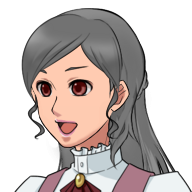
\includegraphics[width=\textwidth]{./jumpakuasset/A.png}\caption{恵伊}\label{fig:jumpakuA}\end{minipage}
\begin{minipage}{0.2\textwidth}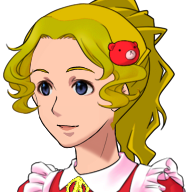
\includegraphics[width=\textwidth]{./jumpakuasset/B.png}\caption{美衣}\label{fig:jumpakuB}\end{minipage}
\begin{minipage}{0.2\textwidth}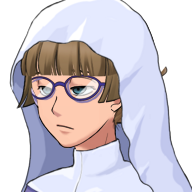
\includegraphics[width=\textwidth]{./jumpakuasset/C.png}\caption{史衣}\label{fig:jumpakuC}\end{minipage}
\begin{minipage}{0.2\textwidth}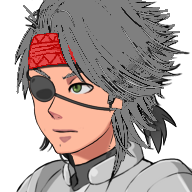
\includegraphics[width=\textwidth]{./jumpakuasset/D.png}\caption{出井}\label{fig:jumpakuD}\end{minipage}\\
\begin{minipage}{0.2\textwidth}
\includegraphics[width=\textwidth]{./jumpakuasset/E.png}\caption{良威}\label{fig:jumpakuE}\end{minipage}
\begin{minipage}{0.2\textwidth}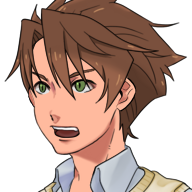
\includegraphics[width=\textwidth]{./jumpakuasset/F.png}\caption{恵夫}\label{fig:jumpakuF}\end{minipage}
\begin{minipage}{0.2\textwidth}
\includegraphics[width=\textwidth]{./jumpakuasset/G.png}\caption{寺井}\label{fig:jumpakuG}\end{minipage}
\begin{minipage}{0.2\textwidth}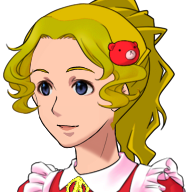
\includegraphics[width=\textwidth]{./jumpakuasset/B.png}\caption{永一}\label{fig:jumpakuH}\end{minipage}\\
\begin{minipage}{0.2\textwidth}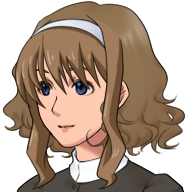
\includegraphics[width=\textwidth]{./jumpakuasset/Me.png}\caption{愛}\label{fig:jumpakuI}\end{minipage}
\begin{minipage}{0.2\textwidth}
\includegraphics[width=\textwidth]{./jumpakuasset/JumpakuMark_250x250.png}\caption{Jumpaku}\label{fig:jumpakuJ}\end{minipage}
\end{tabular}
\end{figure}
彼らの詳しい過去についてはここでは省略するが
\footnote{\href{http://jumpaku.hatenablog.com/entry/2016/04/14/002437}{\underline{愛と血の\ruby[g]{修羅場}{サスペンス}}},
\href{http://jumpaku.hatenablog.com/entry/2016/07/24/032632}{\underline{恋と友情の\ruby[g]{常識}{ファイト}}}および
\href{http://jumpaku.hatenablog.com/entry/2017/07/24/044918}{\underline{罪と幸せの\ruby[g]{四苦八苦}{ノアズアーク}}}をプレイしてください.},
既にこのうち5人が死んでいる.
まず,寺井が恵夫に殺された.
次に,良威が恵伊に殺され,私は報復した.
さらに,恵夫が史衣に殺され,私はまた報復した.
残ったのは,私,美衣,出井,永一の4人だけだった.

美衣,出井,永一の関係を簡単に紹介しておく.
美衣と永一は2人の人格で1つの体を共有しているが,私は2人として扱っている.
また,美衣と永一は姉弟である.
そして,出井と美衣はこの前結婚した.
彼らは生きる希望に満ち溢れていた.

\section{愛の事件}
それはまさに不可能犯罪だった.
密室にいた美衣,出井,永一の3人が消された.
跡形もなく消滅していた.
どのようにそれがなされたのかは分からないし,解明されることも無いだろう.
現場に残されたのはは血文字で書かれた不完全なダイイングメッセージだけだった.

「犯人は...」

\section{愛の決意}
事実は小説より奇なり.
密室より人間が消失した.
現実の世界でそんなことが発生するのだろうか?
いや,しない.
私が現実だと思って生きてきたこの世界は,夢,ゲームまたは小説の中の世界なのかもしれない.
それは,人間が密室から消えるという事象は現実に発生するとは考えられないからだ.
現実の世界で発生しえない事象が発生したなら,その世界は現実の世界ではない.
逆に,この世界が現実ではないとすると,現実で発生しえない事象でも発生しうる.
世界の枠組みを考え直せば,不可能なものが可能となることがあるのだ.
例えば,現実の世界という枠組みの中では人が消える事は無いが,もし小説の世界という枠組みなら人が消えることもある.
私がこれまで現実と思ってきた世界は,実は小説の世界なのかもしれない.
これを現実と確かめる事はできない.
まさに胡蝶の夢である.

しかし,真実を追い求める探偵は,世界の枠組みを考え直すだけで変わってしまうような些細なことに惑わされてはいけない.
探偵が真実を求める際に武器にできるのは論理的な推論しか無いのだ.
前提条件から論理的に推論された結論は,例えこの世界がどのような世界であっても揺らがない.
そのような結論が,探偵が追い求めるべき真実なのだ.
例え,犯人が未登場の者,中国人,探偵自身,双子,複数犯,捜査員,端役,プロの犯罪者または被害者自身であったとしても,
例え,犯行が秘密の通路もしくは隠し部屋,未発見の毒薬,難解な説明を要し,もしくは未来に登場する科学技術または超自然の術によって行われたとしても,
例え,動機が不明瞭であったり,状況に説得力が無かったとしても,
探偵は論理的な推論によって結論を導き,これを真相としなくてはいけない.

\section{愛の推理}
誰かが3人を消したのか?
それとも,3人の中の誰かが犯人で,被害者を消した後,隠れ続けているのか?
まず,私は犯行機会のあった容疑者として私自身,美衣,出井,永一の4人を挙げた.

その上で,美衣と永一が2心同体であったこと,
出井と美衣が愛し合っていたこと,
自分の行動の記憶,
その他3人の性格等を考慮した結果,以下の主張が成り立つと結論付けた.
\begin{itemize}
\item 私は犯人ではなく被害者でもない.
\item 美衣が犯人ならば永一も犯人である.
\item 美衣が被害者ならば永一も被害者である.
\item 容疑者のうち犯人であり被害者でもある者はいない.
\item 容疑者のうち犯人または被害者である者は3人である.
\item 出井は犯人ではない.
\item 美衣が犯人ならば出井は被害者ではない.
\end{itemize}

これらの主張に基づいて,私は上の容疑者のうち犯人は誰なのか,容疑者のうち被害者は誰なのか,
といった真相を論理的に導いた\footnote{ヒントとして,真実を導くプログラムの例を\ref{section:jumpakuprogram}に示す.}.
\begin{description}
\item[容疑者のうち犯人は愛であり, 被害者は出井である.] \ref{section:jumpakufailure1}へ進む.
\item[容疑者のうち犯人は愛であり, 被害者は出井,愛である.] \ref{section:jumpakufailure2}へ進む.
\item[容疑者のうち犯人は愛であり, 被害者は美衣,出井,永一である.] \ref{section:jumpakufailure3}へ進む.
\item[容疑者のうち犯人は永一であり, 被害者は愛である.] \ref{section:jumpakufailure4}へ進む.
\item[容疑者のうち犯人は永一であり, 被害者は美衣,愛である.] \ref{section:jumpakufailure5}へ進む.
\item[容疑者のうち犯人は永一,愛であり, 被害者は美衣,出井,愛である.] \ref{section:jumpakufailure6}へ進む.
\item[容疑者のうち犯人は出井であり, 被害者は愛である.] \ref{section:jumpakufailure7}へ進む.
\item[容疑者のうち犯人は出井であり, 被害者は出井,永一,愛である.] \ref{section:jumpakufailure8}へ進む.
\item[容疑者のうち犯人は出井,愛であり, 被害者は愛である.] \ref{section:jumpakufailure9}へ進む.
\item[容疑者のうち犯人は出井,永一であり, 被害者は美衣である.] \ref{section:jumpakufailure10}へ進む.
\item[容疑者のうち犯人は出井,永一,愛であり, 被害者は出井,永一,愛である.] \ref{section:jumpakufailure11}へ進む.
\item[容疑者のうち犯人は美衣,永一であり, 被害者は美衣,永一である.] \ref{section:jumpakufailure12}へ進む.
\item[容疑者のうち犯人は美衣,永一であり, 被害者は美衣,出井である.] \ref{section:jumpakufailure13}へ進む.
\item[容疑者のうち犯人は美衣,永一,愛であり, 被害者は美衣,愛である.] \ref{section:jumpakufailure14}へ進む.
\item[容疑者のうち犯人は美衣,永一,愛であり, 被害者は美衣,出井である.] \ref{section:jumpakufailure15}へ進む.
\item[容疑者のうち犯人は美衣,出井であり, 被害者は出井である.] \ref{section:jumpakufailure16}へ進む.
\item[容疑者のうち犯人は美衣,出井であり, 被害者は出井,永一である.] \ref{section:jumpakufailure17}へ進む.
\item[容疑者のうち犯人は美衣,出井,愛であり, 被害者は愛である.] \ref{section:jumpakufailure18}へ進む.
\item[容疑者のうち犯人は美衣,出井,愛であり, 被害者は美衣,出井,愛である.] \ref{section:jumpakufailure19}へ進む.
\item[容疑者のうち犯人は美衣,出井,永一であり, 被害者は美衣,出井である.] \ref{section:jumpakufailure20}へ進む.
\item[容疑者のうち犯人は美衣,出井であり, 被害者はいない.] \ref{section:jumpakufailure21}へ進む.
\item[容疑者の中に犯人はおらず,容疑者のうち被害者は美衣,出井,永一である.] \ref{section:jumpakusuccess23}へ進む.
\item[容疑者の中に犯人は美衣,出井,永一であり,容疑者のうち被害者はいない.] \ref{section:jumpakufailure24}へ進む.
\item[容疑者の中に犯人はおらず,容疑者のうち被害者もいない.] \ref{section:jumpakufailure25}へ進む.
\item[容疑者のうち犯人はおらず, 被害者は永一である.] \ref{section:jumpakufailure26}へ進む.
\item[容疑者のうち犯人はおらず, 被害者は出井,永一である.] \ref{section:jumpakufailure27}へ進む.
\end{description}
\newpage

\subsection{失敗}\label{section:jumpakufailure1}間違えた.探偵失敗だ.失敗END...\ref{section:jumpakubegin}へ戻る.\newpage
\subsection{失敗}\label{section:jumpakufailure2}間違えた.探偵失敗だ.失敗END...\ref{section:jumpakubegin}へ戻る.\newpage
\subsection{失敗}\label{section:jumpakufailure3}間違えた.探偵失敗だ.失敗END...\ref{section:jumpakubegin}へ戻る.\newpage
\subsection{失敗}\label{section:jumpakufailure4}間違えた.探偵失敗だ.失敗END...\ref{section:jumpakubegin}へ戻る.\newpage
\subsection{失敗}\label{section:jumpakufailure5}間違えた.探偵失敗だ.失敗END...\ref{section:jumpakubegin}へ戻る.\newpage
\subsection{失敗}\label{section:jumpakufailure6}間違えた.探偵失敗だ.失敗END...\ref{section:jumpakubegin}へ戻る.\newpage
\subsection{失敗}\label{section:jumpakufailure7}間違えた.探偵失敗だ.失敗END...\ref{section:jumpakubegin}へ戻る.\newpage
\subsection{失敗}\label{section:jumpakufailure8}間違えた.探偵失敗だ.失敗END...\ref{section:jumpakubegin}へ戻る.\newpage
\subsection{失敗}\label{section:jumpakufailure9}間違えた.探偵失敗だ.失敗END...\ref{section:jumpakubegin}へ戻る.\newpage
\subsection{失敗}\label{section:jumpakufailure10}間違えた.探偵失敗だ.失敗END...\ref{section:jumpakubegin}へ戻る.\newpage
\subsection{失敗}\label{section:jumpakufailure11}間違えた.探偵失敗だ.失敗END...\ref{section:jumpakubegin}へ戻る.\newpage
\subsection{失敗}\label{section:jumpakufailure12}間違えた.探偵失敗だ.失敗END...\ref{section:jumpakubegin}へ戻る.\newpage
\subsection{失敗}\label{section:jumpakufailure13}間違えた.探偵失敗だ.失敗END...\ref{section:jumpakubegin}へ戻る.\newpage
\subsection{失敗}\label{section:jumpakufailure14}間違えた.探偵失敗だ.失敗END...\ref{section:jumpakubegin}へ戻る.\newpage
\subsection{失敗}\label{section:jumpakufailure15}間違えた.探偵失敗だ.失敗END...\ref{section:jumpakubegin}へ戻る.\newpage
\subsection{失敗}\label{section:jumpakufailure16}間違えた.探偵失敗だ.失敗END...\ref{section:jumpakubegin}へ戻る.\newpage
\subsection{失敗}\label{section:jumpakufailure17}間違えた.探偵失敗だ.失敗END...\ref{section:jumpakubegin}へ戻る.\newpage
\subsection{失敗}\label{section:jumpakufailure18}間違えた.探偵失敗だ.失敗END...\ref{section:jumpakubegin}へ戻る.\newpage
\subsection{失敗}\label{section:jumpakufailure19}間違えた.探偵失敗だ.失敗END...\ref{section:jumpakubegin}へ戻る.\newpage
\subsection{失敗}\label{section:jumpakufailure20}間違えた.探偵失敗だ.失敗END...\ref{section:jumpakubegin}へ戻る.\newpage
\subsection{失敗}\label{section:jumpakufailure21}間違えた.探偵失敗だ.失敗END...\ref{section:jumpakubegin}へ戻る.\newpage
\subsection{失敗}\label{section:jumpakufailure22}間違えた.探偵失敗だ.失敗END...\ref{section:jumpakubegin}へ戻る.\newpage
\subsection{成功}\label{section:jumpakusuccess23}真実へ到達した.\ref{section:jumpakuresult}へ進む.\newpage
\subsection{失敗}\label{section:jumpakufailure24}間違えた.探偵失敗だ.失敗END...\ref{section:jumpakubegin}へ戻る.\newpage
\subsection{失敗}\label{section:jumpakufailure25}間違えた.探偵失敗だ.失敗END...\ref{section:jumpakubegin}へ戻る.\newpage
\subsection{失敗}\label{section:jumpakufailure26}間違えた.探偵失敗だ.失敗END...\ref{section:jumpakubegin}へ戻る.\newpage
\subsection{失敗}\label{section:jumpakufailure27}間違えた.探偵失敗だ.失敗END...\ref{section:jumpakubegin}へ戻る.\newpage

\section{愛の真相}\label{section:jumpakuresult}
真犯人は容疑者の中にはいない.
美衣,出井,永一は全員被害者だ.
これは論理的に導かれるたった一つの真相である.
例え,どんな理由があろうとも,
論理的な推論によって導かれる結論なのだから,これは真実なのだ.

\section{愛の飛躍}
探偵としての仕事が終わった.
ところが,私の思考は続いた.
失った仲間を思うと思考せずにはいられなかった.
3人を消した犯人は容疑者の中にはいない.
では,それ以外の誰なのか?
その思考は論理的な推論を飛躍した.

そもそも,
\begin{description}
\item[この世界は現実ではない.] \ref{subsection:jumpakulast1success}へ進む.
\item[この世界は現実である.] \ref{subsection:jumpakulast1failure}へ進む.
\end{description}
\newpage

\subsection{成功}\label{subsection:jumpakulast1success}なぜなら,密室から人間が消失する事は現実の世界では発生しないのだから.
次に,現実ではないこの世界は
\begin{description}
\item[何者かの意思によって作り出されている気がする.] \ref{subsection:jumpakulast2success}へ進む.
\item[ランダムに生成されている気がする.] \ref{subsection:jumpakulast2failure}へ進む.
\end{description}
\newpage

\subsection{失敗}\label{subsection:jumpakulast1failure}\ref{section:jumpakubegin}へ戻る.\newpage

\subsection{成功}\label{subsection:jumpakulast2success}
なぜなら,私の周りで殺人事件が多すぎること,
私を含めた仲間の名前がアルファベット順に並ぶことなど,不自然なことが多いから.

この世界を作り,私の仲間を消した犯人の名前の頭文字は
\begin{description}
\item[A] \ref{subsection:jumpakulast3failureA}へ進む.
\item[B] \ref{subsection:jumpakulast3failureB}へ進む.
\item[C] \ref{subsection:jumpakulast3failureC}へ進む.
\item[D] \ref{subsection:jumpakulast3failureD}へ進む.
\item[E] \ref{subsection:jumpakulast3failureE}へ進む.
\item[F] \ref{subsection:jumpakulast3failureF}へ進む.
\item[G] \ref{subsection:jumpakulast3failureG}へ進む.
\item[H] \ref{subsection:jumpakulast3failureH}へ進む.
\item[I] \ref{subsection:jumpakulast3failureI}へ進む.
\item[J] \ref{subsection:jumpakulast3successJ}へ進む.
\item[K] \ref{subsection:jumpakulast3failureK}へ進む.
\item[L] \ref{subsection:jumpakulast3failureL}へ進む.
\item[M] \ref{subsection:jumpakulast3failureM}へ進む.
\item[N] \ref{subsection:jumpakulast3failureN}へ進む.
\item[O] \ref{subsection:jumpakulast3failureO}へ進む.
\item[P] \ref{subsection:jumpakulast3failureP}へ進む.
\item[Q] \ref{subsection:jumpakulast3failureQ}へ進む.
\item[R] \ref{subsection:jumpakulast3failureR}へ進む.
\item[S] \ref{subsection:jumpakulast3failureS}へ進む.
\item[T] \ref{subsection:jumpakulast3failureT}へ進む.
\item[U] \ref{subsection:jumpakulast3failureU}へ進む.
\item[V] \ref{subsection:jumpakulast3failureV}へ進む.
\item[W] \ref{subsection:jumpakulast3failureW}へ進む.
\item[X] \ref{subsection:jumpakulast3failureX}へ進む.
\item[Y] \ref{subsection:jumpakulast3failureY}へ進む.
\item[Z] \ref{subsection:jumpakulast3failureZ}へ進む.
\end{description}
\newpage

\subsection{失敗}\label{subsection:jumpakulast2failure}\ref{section:jumpakubegin}へ戻る.\newpage

\subsection{失敗}\label{subsection:jumpakulast3failureA}\ref{section:jumpakubegin}へ戻る.\newpage
\subsection{失敗}\label{subsection:jumpakulast3failureB}\ref{section:jumpakubegin}へ戻る.\newpage
\subsection{失敗}\label{subsection:jumpakulast3failureC}\ref{section:jumpakubegin}へ戻る.\newpage
\subsection{失敗}\label{subsection:jumpakulast3failureD}\ref{section:jumpakubegin}へ戻る.\newpage
\subsection{失敗}\label{subsection:jumpakulast3failureE}\ref{section:jumpakubegin}へ戻る.\newpage
\subsection{失敗}\label{subsection:jumpakulast3failureF}\ref{section:jumpakubegin}へ戻る.\newpage
\subsection{失敗}\label{subsection:jumpakulast3failureG}\ref{section:jumpakubegin}へ戻る.\newpage
\subsection{失敗}\label{subsection:jumpakulast3failureH}\ref{section:jumpakubegin}へ戻る.\newpage
\subsection{失敗}\label{subsection:jumpakulast3failureI}\ref{section:jumpakubegin}へ戻る.\newpage
\subsection{成功}\label{subsection:jumpakulast3successJ}\ref{section:jumpakuending}へ進む.\newpage
\subsection{失敗}\label{subsection:jumpakulast3failureK}\ref{section:jumpakubegin}へ戻る.\newpage
\subsection{失敗}\label{subsection:jumpakulast3failureL}\ref{section:jumpakubegin}へ戻る.\newpage
\subsection{失敗}\label{subsection:jumpakulast3failureM}\ref{section:jumpakubegin}へ戻る.\newpage
\subsection{失敗}\label{subsection:jumpakulast3failureN}\ref{section:jumpakubegin}へ戻る.\newpage
\subsection{失敗}\label{subsection:jumpakulast3failureO}\ref{section:jumpakubegin}へ戻る.\newpage
\subsection{失敗}\label{subsection:jumpakulast3failureP}\ref{section:jumpakubegin}へ戻る.\newpage
\subsection{失敗}\label{subsection:jumpakulast3failureQ}\ref{section:jumpakubegin}へ戻る.\newpage
\subsection{失敗}\label{subsection:jumpakulast3failureR}\ref{section:jumpakubegin}へ戻る.\newpage
\subsection{失敗}\label{subsection:jumpakulast3failureS}\ref{section:jumpakubegin}へ戻る.\newpage
\subsection{失敗}\label{subsection:jumpakulast3failureT}\ref{section:jumpakubegin}へ戻る.\newpage
\subsection{失敗}\label{subsection:jumpakulast3failureU}\ref{section:jumpakubegin}へ戻る.\newpage
\subsection{失敗}\label{subsection:jumpakulast3failureV}\ref{section:jumpakubegin}へ戻る.\newpage
\subsection{失敗}\label{subsection:jumpakulast3failureW}\ref{section:jumpakubegin}へ戻る.\newpage
\subsection{失敗}\label{subsection:jumpakulast3failureX}\ref{section:jumpakubegin}へ戻る.\newpage
\subsection{失敗}\label{subsection:jumpakulast3failureY}\ref{section:jumpakubegin}へ戻る.\newpage
\subsection{失敗}\label{subsection:jumpakulast3failureZ}\ref{section:jumpakubegin}へ戻る.\newpage

\section{愛の終点}\label{section:jumpakuending}
私の世界を作り,私を生かし,仲間を奪ったのはこの物語を書いたJumpakuである.
動機はきっと「面白いと思ったから」だろう.
私は世界の理を理解した.

そして.

それでも.

もっと,生きよう.

解決END.
\newpage

\section*{サンプルコード}\label{section:jumpakuprogram}
以下に今回の事件の論理的推論を行うためのPython3のプログラムを示す.
\inputminted[linenos]{python3}{./jumpakuasset/LogicQuiz.py}

\section*{あとがき}
本章にはBSD 2-Clause Licenseが適用されます.

\begin{quote}
BSD 2-Clause License

Copyright (c) 2018, Jumpaku
All rights reserved.

Redistribution and use in source and binary forms, with or without
modification, are permitted provided that the following conditions are met:
\begin{itemize}
\item Redistributions of source code must retain the above copyright notice, this
  list of conditions and the following disclaimer.
\item Redistributions in binary form must reproduce the above copyright notice,
  this list of conditions and the following disclaimer in the documentation
  and/or other materials provided with the distribution.
\end{itemize}
THIS SOFTWARE IS PROVIDED BY THE COPYRIGHT HOLDERS AND CONTRIBUTORS "AS IS"
AND ANY EXPRESS OR IMPLIED WARRANTIES, INCLUDING, BUT NOT LIMITED TO, THE
IMPLIED WARRANTIES OF MERCHANTABILITY AND FITNESS FOR A PARTICULAR PURPOSE ARE
DISCLAIMED. IN NO EVENT SHALL THE COPYRIGHT HOLDER OR CONTRIBUTORS BE LIABLE
FOR ANY DIRECT, INDIRECT, INCIDENTAL, SPECIAL, EXEMPLARY, OR CONSEQUENTIAL
DAMAGES (INCLUDING, BUT NOT LIMITED TO, PROCUREMENT OF SUBSTITUTE GOODS OR
SERVICES; LOSS OF USE, DATA, OR PROFITS; OR BUSINESS INTERRUPTION) HOWEVER
CAUSED AND ON ANY THEORY OF LIABILITY, WHETHER IN CONTRACT, STRICT LIABILITY,
OR TORT (INCLUDING NEGLIGENCE OR OTHERWISE) ARISING IN ANY WAY OUT OF THE USE
OF THIS SOFTWARE, EVEN IF ADVISED OF THE POSSIBILITY OF SUCH DAMAGE.
\end{quote}

また,キャラクタの画像は罪と幸せの\ruby[g]{四苦八苦}{ノアズアーク}より引用しました.

\newpage
\myimpression
\end{document}
